\documentclass{if-beamer}
\usepackage{tikz-cd}
\newcommand{\MR}[1]{\href{http://www.ams.org/mathscinet-getitem?mr=#1}{MR#1}}
% --------------------------------------------------- %
%                  Presentation info	              %
% --------------------------------------------------- %
\title[Branching Random Walk in Random Environment]{Branching Random Walk in Random Environment}
\author[Liu]{Xiaoyu Liu} % Add the second author here
\institute[Purdue]{Purdue University \and \textbf{Mentors: Prof. Jonathon Peterson (Purdue)}}


    
\begin{document}

\begin{frame}
  \titlepage
\end{frame}

\section{Simple RW}


\begin{frame}{Random Motion}
    \begin{figure}
        \centering
        
\includegraphics[width=0.7\textwidth]{figures/brownian_motion_2d.png}
        % \caption{Process 2}
    \end{figure}
\end{frame}


\begin{frame}{A physical perspective}
    \begin{columns}
        \begin{column}{0.5\textwidth}
            \begin{figure}
                \centering
                
\includegraphics[width=\textwidth]{figures/gaussian_samples_2d.png}
                % \caption{Process 1}
            \end{figure}
        \end{column}
        \begin{column}{0.5\textwidth}
            \begin{figure}
                \centering
                
\includegraphics[width=\textwidth]{figures/heat_kernel_2d.png}
                % \caption{Process 2}
            \end{figure}
        \end{column}
    \end{columns}
\end{frame}

\begin{frame}{A physical perspective}
    \begin{columns}
        \begin{column}{0.5\textwidth}
            \begin{block}{Heat semigroup}
                Time-evolution of a diffusion process, irreversible.
            \end{block}
            % space
            \vspace{1em}
            Ensemble Average
            \begin{equation*}
                \frac{1}{N} \sum_{i = 1}^N f(X^{(i)}_t) \xrightarrow{N \to \infty} \mathbb{E}[f(X_t)] = H_t f 
            \end{equation*}

            % space
            \vspace{1em}

            \begin{block}{Brownian Motion}
                Microscopic model of particles in heat motion, reversible.
            \end{block}
            
        \end{column}
        \begin{column}{0.5\textwidth}
            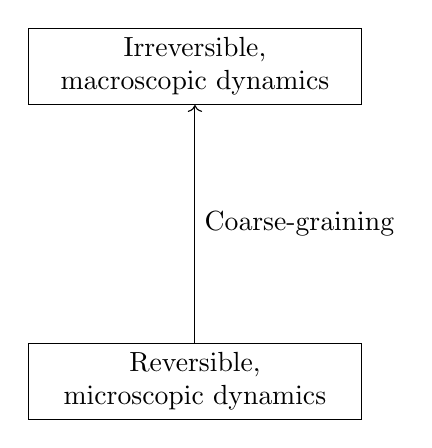
\begin{tikzpicture}
                \node (A) at (0,0) [draw, rectangle, text width=4cm, align=center] {Reversible,\\ microscopic dynamics};
                \node (B) at (0,4) [draw, rectangle, text width=4cm, align=center] {Irreversible,\\ macroscopic dynamics};
                \draw[->] (A) -- (B) node[midway, right] {Coarse-graining};
            \end{tikzpicture}
            
            
        \end{column}
    \end{columns}
\end{frame}


\begin{frame}{Simple Random Walk in One Dimension}

    % two columns
    \begin{columns}
        \begin{column}{0.6\textwidth}
            \begin{block}{Definition}
                \begin{itemize}
                    \item $X_k$ is a random walk on $\mathbb{Z}^1$. At each step, it moves to the left or right.
                \end{itemize}
            \end{block}
        \end{column}
        \begin{column}{0.5\textwidth}
            % figure
            \begin{figure}
                \centering
                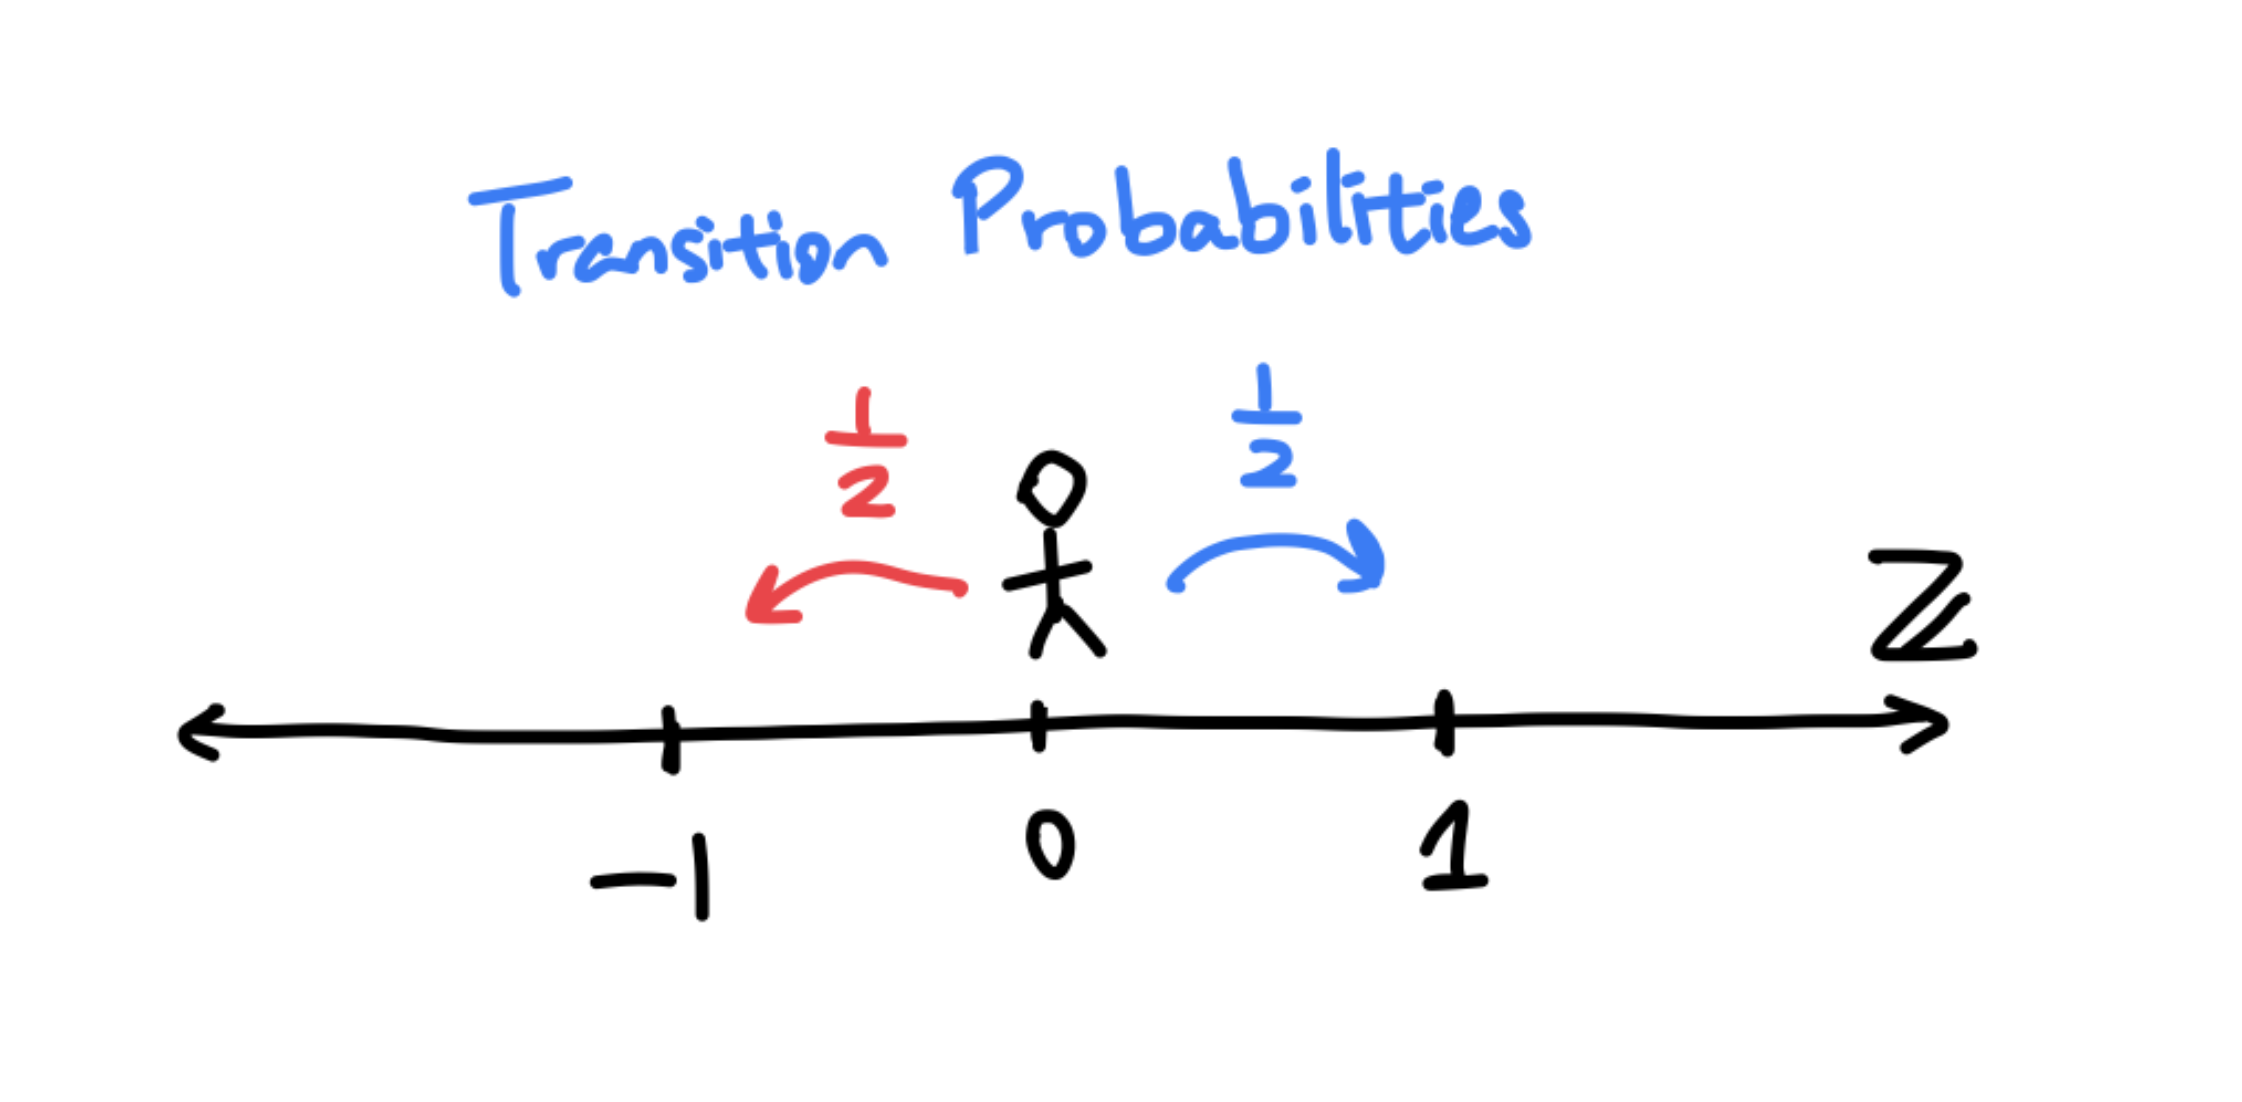
\includegraphics[width=0.7\textwidth]{src/doodle-def1.png}
            \end{figure}
        \end{column}
    \end{columns}

\end{frame}



\begin{frame}{Scaling Limit}
        \begin{minipage}{0.45\textwidth}
            \centering
            
\includegraphics[width=\textwidth]{figures/srw_x1.png}<1>
            
\includegraphics[width=\textwidth]{figures/srw_x2.png}<2>
            
\includegraphics[width=\textwidth]{figures/srw_x3.png}<3>
            
\includegraphics[width=\textwidth]{figures/srw_x4.png}<4->
        \end{minipage}
        \begin{math}
        \uncover<6->{\frac{X_{nt}}{\sqrt{n}} \xrightarrow{n \to \infty} B_t}
        \end{math}
        \begin{minipage}{0.45\textwidth}
            \centering
            
\includegraphics[width=\textwidth]{figures/srw_x5.png}<5->
        \end{minipage}
    % three parallel text blocks
    \begin{block}<7->{Good to know}
        \begin{columns}
            % 3 columns
            \begin{column}{0.3\textwidth}
                \begin{itemize}
                    \item 
                    $ B_t - B_s \sim \mathcal{N}(0, t-s)$
                    \item Markov process
                \end{itemize}
            \end{column}
            \begin{column}{0.3\textwidth}
                \begin{itemize}
                    \item $E(X_{t + s} | X_s) = X_s$
                    \item Martinagle
                \end{itemize}
            \end{column}
            \begin{column}{0.3\textwidth}
                \begin{itemize}
                    \item Visits every point infinitely often
                    \item Recurrent
                \end{itemize}
            \end{column}
        \end{columns}
    \end{block}

    \begin{alertblock}<8->{Question}
        \begin{itemize}
            \item What if there's heterogeneous environment?
            % \item What if $X_k$ is not Markovian?
            \item What if $X_k$ is a branching walk?
        \end{itemize}
    \end{alertblock}
\end{frame}

\begin{frame}{Range and Speedup of simple RW}
     % two columns
     \begin{columns}
        \begin{column}{0.6\textwidth}
            \begin{block}{Fact}
                \begin{itemize}
                    \item<1-> Brownian Scaling: 
                    \begin{equation*}
                        \frac{X_{nt}}{\sqrt{n}} \xrightarrow{n \to \infty} B_t
                    \end{equation*}
                    \item<2-> The range of $X_k$ grows like $O(\sqrt{k})$.
                    \item<3-> That is, it has \emph{zero speed}: $\lim_{k \to \infty} \frac{X_k}{k} = 0$.
                \end{itemize}
            \end{block}
            \begin{block}<4->{Speedup}
                \begin{itemize}
                    \item<4-> Can $X_k$ be about $x k$ for some $x \neq 0$?
                    \item<5-> Probability for $X_k = k$, i.e., $x = 1$:
                    \[
                    P\left(X_k = k\right)=2^{-k}
                    \]
                    \[
                    \lim_{k \to \infty} \frac{1}{k} \log P\left(X_k = k\right) = - \log 2
                    \]  
                \end{itemize}
            \end{block}
        \end{column}
        \begin{column}{0.5\textwidth}
            \begin{figure}
                \centering
                \includegraphics<2->[width=0.8\textwidth]{figures/bm_1d_many.png}
            \end{figure}
            \begin{figure}
                \centering
                \includegraphics<6>[width=0.8\textwidth]{figures/cramer_rate_function.png}
            \end{figure}

        \end{column}
    \end{columns} 
\end{frame}


% \section{Physical Motivations}


% \begin{frame}{Self-Avoiding Walks}

%     % two images
%     \begin{figure}
%         \centering
%         \begin{minipage}{0.3\textwidth}
%             \centering
%             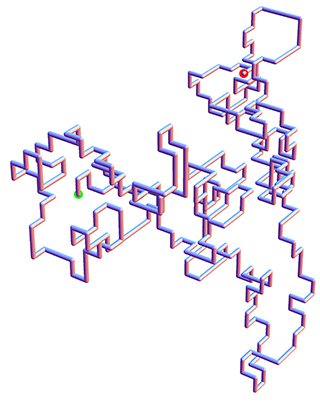
\includegraphics[width=\textwidth]{src/SAW.jpg}
%             \caption{Simulated self-avoiding walk (Math StackOverflow)}
%         \end{minipage}
%         \hfill
%         \begin{minipage}{0.37\textwidth}
%             \centering
%             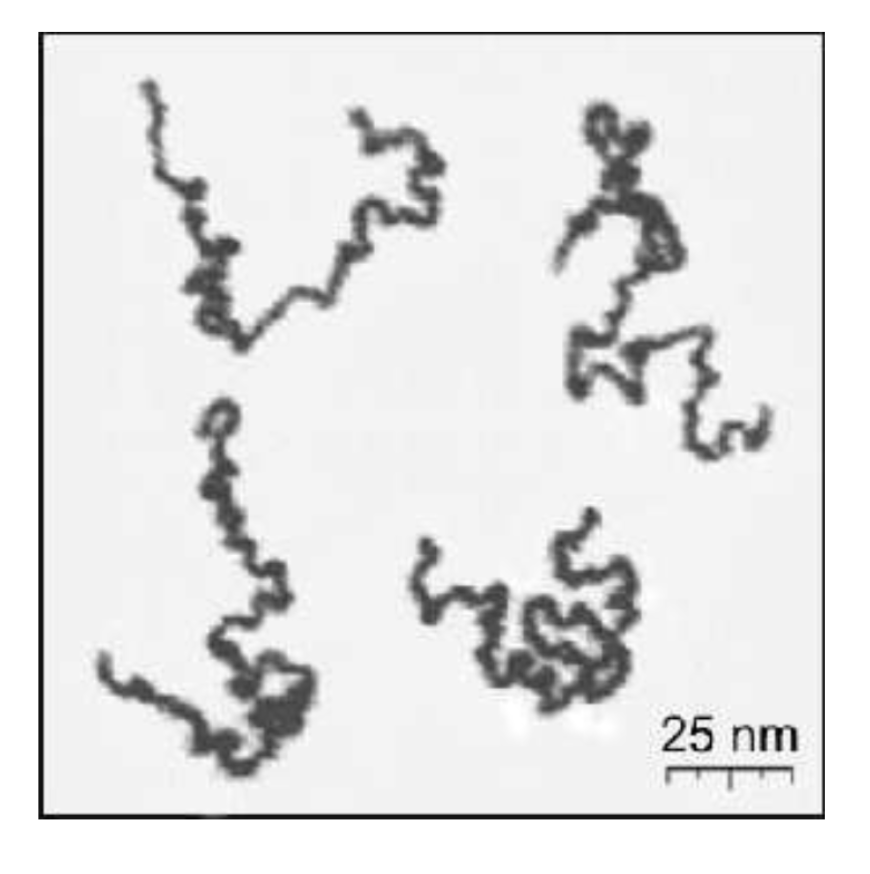
\includegraphics[width=\textwidth]{src/polymer.png}
%             \caption{Polymer chain (Image credit: Roiter and Minko, 2005)}
%         \end{minipage}
%     \end{figure}

% \end{frame}


% \begin{frame}{Feller Semigroups and Feller Process}

%     \begin{columns}
%         \begin{column}{0.5\textwidth}
%             \begin{block}{Feller Semigroup}
%                 A family of operators $P_t$ on $L^p(\mathbb{R}^n)$, $1\leq p\leq \infty$, is a \textbf{Feller semigroup} if
%                 \begin{itemize}
%                     \item $P_t$ is a contraction on $L^p$.
%                     \item $P_t$ is \textit{strongly continuous} in $t$.
%                     \item $P_t$ is \textit{positivity preserving}.
%                 \end{itemize}
%             \end{block}
%             \begin{block}{Feller Process}
%                 A \textbf{Feller process} is a Markov process with a Feller semigroup.
%             \end{block}
%             If $P_t$ is self-adjoint on $L^2$, then the process is \textbf{reversible}.
%             \begin{exampleblock}{Examples}
%                 \begin{itemize}
%                     \item Heat kernel $\longleftrightarrow$ Brownian motion
%                     \item Poisson kernel $\longleftrightarrow$ Cauchy process
%                 \end{itemize}
%             \end{exampleblock}
%         \end{column}
%         \begin{column}{0.5\textwidth}
%             \begin{figure}
%                 \centering
%                 
\includegraphics[width=0.5\textwidth]{figures/heat_kernel_2d.png}
%             \end{figure}
%             \begin{figure}
%                 \centering
%                 
\includegraphics[width=0.5\textwidth]{figures/brownian_motion_2d.png}
%             \end{figure}
%         \end{column}
%     \end{columns}
% \end{frame}




\section{RWRE}

\begin{frame}{Random Walk in Random Environment}
    
    % two columns
    \begin{columns}
        \begin{column}{0.6\textwidth}
            \begin{block}{Definition}
                \begin{itemize}
                    \item Location-dependent transition probabilities:
                    \[
                    P(X_{k + 1} = x + 1 | X_k = x) = \omega_x \in [\kappa, 1 - \kappa]
                    \]
                    \item<2-> $(\omega_x)_{x \in \mathbb{Z}}$ is the \emph{random environment}
                    \item<3-> Assume environment to be i.i.d. or ergodic.
                \end{itemize}
            \end{block}
            \begin{block}<4->{Recurrence and Transience, Ballisticity}
                Not recurrent in general; even if transient, does not have positive speed in general.
            \end{block}
            \begin{block}<5->{Large Deviation Principle}
                LDP for ergodic environment given by Comet et al., 2000. In the right transient ballistic case:
            \end{block}
        \end{column}
        \begin{column}{0.4\textwidth}
            % figure
            \begin{figure}
                \centering
                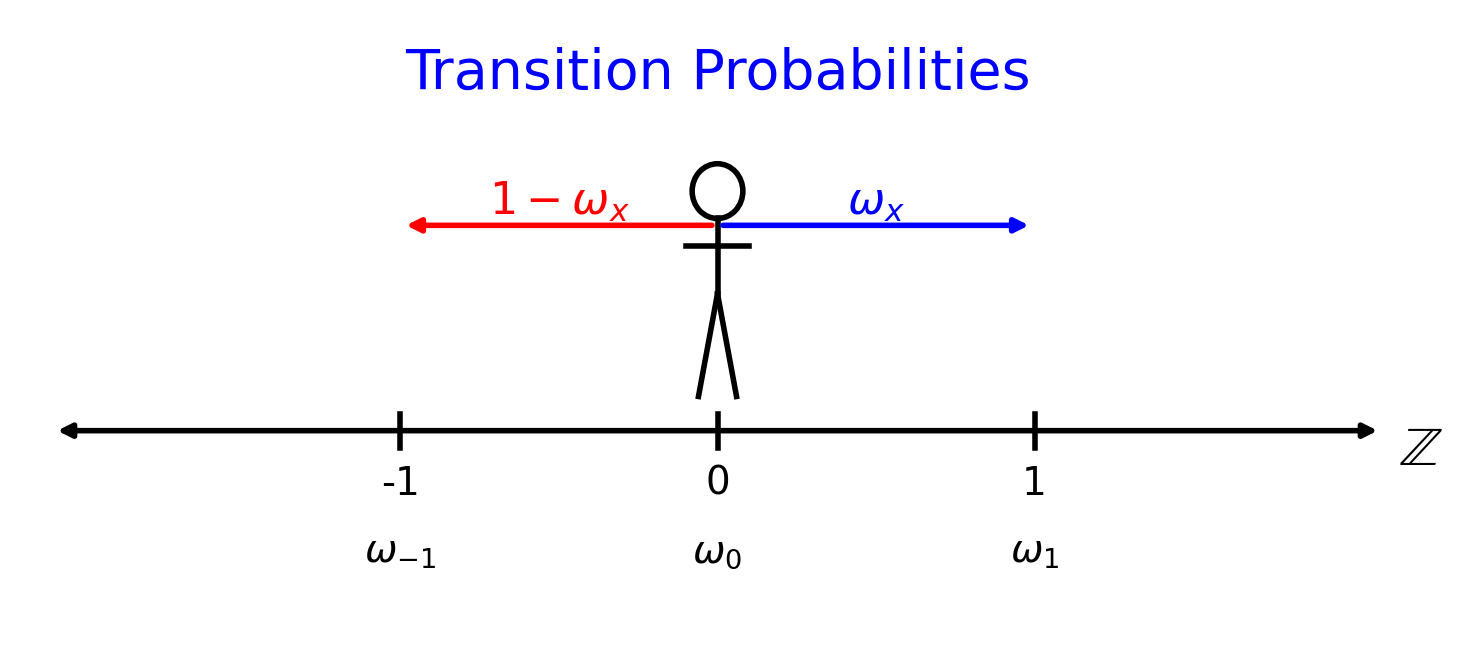
\includegraphics[width=0.7\textwidth]{figures/rwre-def.png}
            \end{figure}
            \begin{figure}
                \centering
                \includegraphics<4->[width=0.7\textwidth]{figures/rwre_10000.png}
            \end{figure}
            \begin{figure}
                \centering
                \includegraphics<5->[width=0.7\textwidth]{src/comet-fig8.png}
            \end{figure}
        \end{column}
    \end{columns}

\end{frame}

\section{BRW}
\begin{frame}{Branching Random Walk}
    \begin{figure}
        \centering
        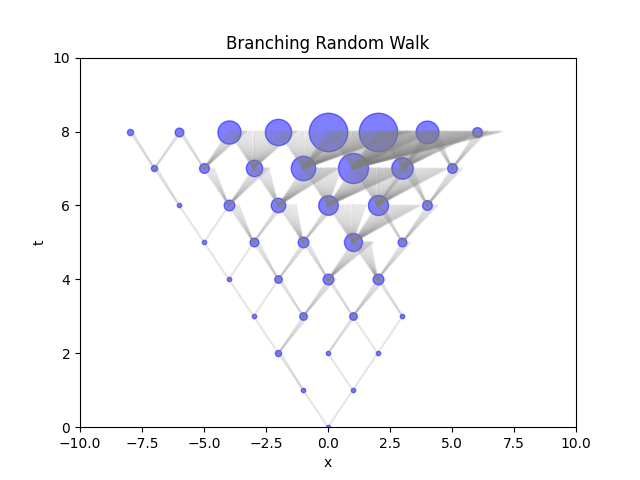
\includegraphics[width=0.7\textwidth]{figures/brw.png}
    \end{figure} 
    \begin{exampleblock}<2>{Speed of Maximum Particle}
        In the branching simple random walk case,
        we have
        $M_n = x^* n - \frac{3\log n}{2 t}+O(1)$, where $x^*$ and $t$ are computed from the branching law.
    \end{exampleblock}
\end{frame}

% \section{More Motivations}

% \begin{frame}{Discrete Processes and Their Continuous Limits}
%     % Grid layout version

%     \begin{tabular}{cc}
%     % First cell: Discrete Process
%     \begin{minipage}{0.45\textwidth}
%         \begin{block}{Discrete Process}
%             \centering
%             
\includegraphics[width=\linewidth]{figures/srw_x4.png}
%         \end{block}
%     \end{minipage}
%     &
%     % Second cell: Continuous Process
%     \begin{minipage}{0.45\textwidth}
%         \begin{block}{Continuous Process}
%             \centering
%             
\includegraphics[width=\linewidth]{figures/srw_x5.png}
%         \end{block}
%     \end{minipage} \\
%     \end{tabular}

   
% \end{frame}



\section{Our Project}

\begin{frame}{Branching Random Walk in Random Environment}
    \begin{columns}
        \begin{column}{0.5\textwidth}
            \begin{exampleblock}{Our Question}
                What is the speed of the maximum particle in a branching random walk in random environment?
            \end{exampleblock}
            \begin{block}<2->{Current Result}
                \[
                M_n = x^* n + o(n)
                \]
                Lower order terms work in progress.
            \end{block}
        \end{column}
        \begin{column}{0.5\textwidth}
            \begin{figure}
                \centering
                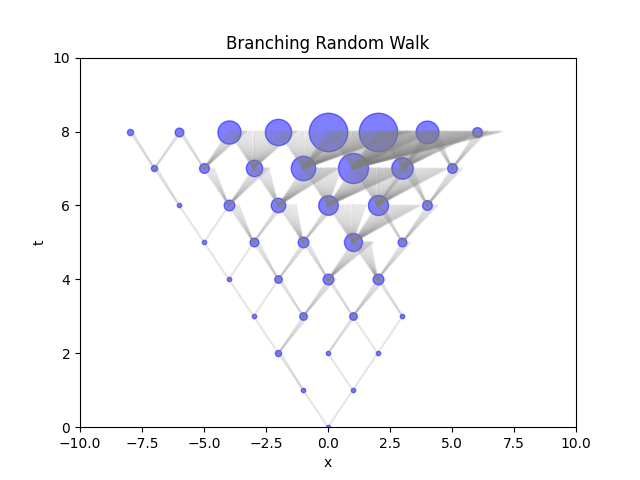
\includegraphics[width=0.7\textwidth]{figures/brw.png}
            \end{figure}  
        \end{column}
    \end{columns}

    \begin{block}<3->{Upper Bound of $x^*$}
        By LDP, $P(M_n \geq x^* n) \lesssim k^n \exp(- n I(x^*))$, which is summable for $I(x^*) > \log k$.

        Hence, a.s., $\limsup \frac{M_n}{n} \leq x^*$.
    \end{block}
    
\end{frame}

\begin{frame}{Lower Bound for $x^*$}
    \begin{block}{Step 1: Coarse Graining}
        Again by LDP, for any $x^*$ such that $I(x^*) < \log k$, expected number of particle achieving this speed is very high:
        \pause
        \[
            \mathbb{E}\left[\log E_\omega[|\{v: v_L - v_0 > x^* L\}|]\right]>0, \quad \text { for large } L
        \]
        \pause
        So we chunk up the space into $L$-sized blocks and only let the particles achieving this speed to survive.
    \end{block}
    \pause
    \begin{columns}
        \begin{column}{0.5\textwidth}
            \begin{block}{Step 2: Realignment and Coupling}
                We want to make events on each piece independent, so we construct a coupling.
            \end{block}
        \end{column}
        \begin{column}{0.5\textwidth}
            \begin{figure}
                \centering
                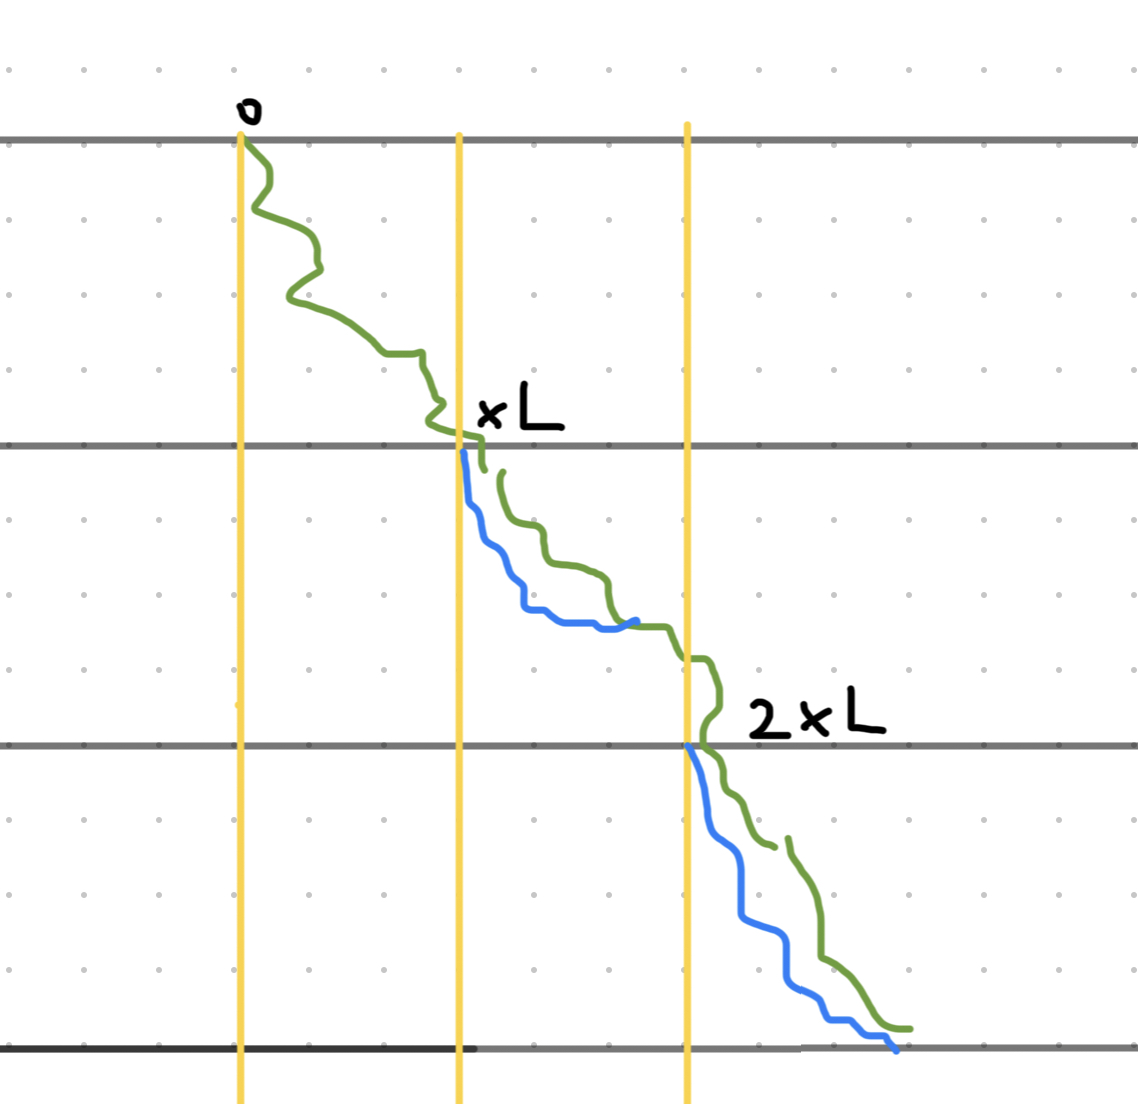
\includegraphics[width=0.7\textwidth]{src/coupling-doodle.png}
            \end{figure}   
        \end{column}
        
    \end{columns}
    
\end{frame}

\begin{frame}{Lower Bound for $x^*$}
    \pause
    \begin{block}{Step 3: Super-criticality}
        Because of Step 1, the coarse-grained tree, that either achieves the speed $x^*$ or dies, is a super-critical branching process.
    \end{block}
    \pause
    \begin{block}{Step 4: Amplification}
        But there are many, many independent copies of this tree, so Borel-Cantelli implies there's at least one such tree.
    \end{block}
    \pause
    \begin{block}{Conclusion}
        \[
            \liminf_{n \to \infty} \frac{M_n}{n} \geq x^* \qquad \text{a.s. for all }
            x^* \text{ such that } I(x^*) < \log k
        \]
        QED.
    \end{block}
\end{frame}

\begin{frame}{Next Steps, Main Ideas}


    Next Steps:

    \begin{itemize}
        \item Try to understand lower-order corrections of the speed of maximal particle.
        \item From that, gather more information about the distribution of the maximum particle.
        \item (Maybe) Look into scaling limits of the branching random walk in random environment.
    \end{itemize}

    \pause
    Main Ideas:

    \begin{itemize}
        \item \emph{Random walks} and ensembles of them help us understand complex physical systems that are important in statistical mechanics.
        \item \emph{Scaling limit} bridges discrete and continuous structures.
    \end{itemize}
\end{frame}

\section{References and Appendix}
\begin{frame}
    \begin{center}
        \Huge Thank you.
    \end{center}
\vfill
    
\begin{itemize}
    \item Athreya, K., \& Karlin, S., \emph{Branching processes with random environments} (1970). \url{https://doi.org/10.1090/S0002-9904-1970-12589-7}

    \item Comets, F., Gantert, N., \& Zeitouni, O., \emph{Quenched, annealed and functional large deviations for one-dimensional random walk in random environment}, Probability Theory and Related Fields \textbf{118} (2000), no.~1, 65–114. \url{https://doi.org/10.1007/s004400000074}

    \item Dembo, A., \& Zeitouni, O., \emph{Large Deviations Techniques and Applications} (Vol. 38), Springer Berlin Heidelberg, 2010. \url{https://doi.org/10.1007/978-3-642-03311-7}

    \item Peterson, J., \emph{Lecture Notes on Random Walks in Random Environments}.

    \item Zeitouni, O., \emph{Branching Random Walks and Gaussian Fields: Notes for Lectures} (2020). Lecture note.

    \end{itemize}
\end{frame}

\end{document}
